\documentclass{llncs}

\usepackage{microtype}
\usepackage{amsmath,amssymb,mathtools}
\usepackage{hyperref}
\usepackage{booktabs}
\usepackage{graphicx}
\usepackage{tablefootnote}
\usepackage[backend=bibtex,firstinits=true]{biblatex}
\addbibresource{paper.bib}
\makeatletter
\def\blx@maxline{77}
\makeatother

\usepackage{pifont}
\newcommand{\cmark}{\ding{51}}%
\newcommand{\xmark}{\ding{55}}%

\newcommand{\etal}{et~al.\@}

\newcommand{\AppPAL}[0]{SP4BYOD}

\usepackage{acronym}
\acrodef{MDM}{Mobile Device Management}
\acrodef{BES}{Blackberry Enterprise Services}
\acrodef{HiMSS}{Healthcare Information Management System Society}

\usepackage{listings}
\lstdefinelanguage{AppPAL}{%
  morekeywords={if,inf,says,where,true,false,with,is},
  otherkeywords={can-act-as,can-say},
  sensitive=true,
  morestring=[b]',
  literate={\ inf\ }{{$\infty$}}5
}[keywords,strings]
\newcommand{\listingsize}[0]{\footnotesize}
\lstset{%
  basicstyle=\normalfont\ttfamily\listingsize,
  keywordstyle=\normalfont\ttfamily\slshape\listingsize,
  stringstyle=\normalfont\sffamily\listingsize,
  columns=flexible,
  mathescape,
  tabsize=2,
  showstringspaces=true,
  %numbers=left,
  frame=single,
  breaklines=true,
  numberstyle=\tiny\ttfamily\color{Gray},
  commentstyle=\ttfamily\color{Gray}
}
\newcommand{\code}[2][]{\lstinline[breaklines=true, #1]{#2}}

\usepackage{mdframed}
\newcommand{\todo}[1]{\marginpar{\begin{mdframed}[userdefinedwidth=1cm]\tiny\sffamily\raggedright #1\end{mdframed}}}

\newenvironment{policyrule}[1]{%
  \begin{mdframed}\footnotesize
      \noindent\textbf{\sffamily #1}:~\itshape%
}{%
  \end{mdframed}
}

\title{Capturing Policies for BYOD}
\author{Joseph Hallett and David Aspinall}
\institute{University of Edinburgh}
\begin{document}
\maketitle
\begin{abstract}
  % 4 Sentences
  BYOD policies are informally specified using natural language.
  Various tools and \ac{MDM} solutions can implement parts of the policies, but there isn't a means to tie the written policy to its enforcement method.
  The \AppPAL~language is shown capturing BYOD policies throughout the paper.
  We identify common BYOD idioms and delegation structures.
\end{abstract}
\section{Introduction}
\label{sec:intro}
% Describe the problem
% State my contribution
% 1 page

Employees bring their own devices to work.
In the past employees might have had a dedicated company device.
Today around 70\% of companies have a BYOD scheme~\cite{schulze_byod_2016} and, in some fields,
  85\% of staff use their personal devices to look up work-sensitive information~\cite{patel_uk_2015}.
Controlling employee's devices is a challenge for IT departments.
They need to control access to company resources but have limited control over the devices used to access them.

One solution to controlling devices is to require users to agree to follow policies.
They often take the form of a user agreement, written in natural language, which describes how the devices should be used and configured.
Various guides are available for companies wishing to implement a policy from governments, standards bodies, and organizations seeking to advise~\cite{nicholas_r._c._guerin_security_2008,souppaya_guidelines_????,hp_byod_????,cesg_byod_2015}.
On top of user agreements, companies may also use \ac{MDM} software; which can enforce policies.
But the use of \ac{MDM} software does not guarantee compliance.
One survey found over 50\% of companies with \ac{MDM} software have devices that do not comply with their policies in their networks~\cite{mobileiron_security_labs_q4_2015}.

The policies are becoming more intricate.
\ac{MDM} software is becoming more proficient.
There has been much work looking at developing the \ac{MDM} software to enforce aspects of BYOD policies~\cite{costantino_towards_2013,martinelli_enhancing_2016,armando_enabling_2014}.
Implementing a policy is only part of the problem, however.
BYOD policies are specified informally using natural language, and they contain more than just access control decisions.
These policies describe trust relationships inside the company between the IT departments, users, and HR each who may be delegated to make decisions and provide rules.
Policies contain rules that require employees to acknowledge risks, and regulations.
An antivirus or \ac{MDM} program may be used to \emph{implement} part of the policy.
But it is the policy, however, that \emph{specifies} which software to use and when. 
There is no automatic way to check how the policy has been implemented and by what.

Using a formalization of five BYOD policies written using \AppPAL~we identify different idioms and common delegation patterns present in BYOD policies.
Our formalizations pick out the common concerns and trust relationships in these policies.
We look at what decisions and trust relationships used in BYOD policies.
These are BYOD idioms that are capture decisions and frequently seen requirements in BYOD policies.
These give a guide for where future work implementing BYOD tools should focus their efforts to cover more aspects of policies.

We show how \AppPAL~can be used to implement these policies and describe precisely the different trust relationships.
\AppPAL~is an instantiation of the SecPAL authorization language~\cite{becker_secpal:_2010} for mobile device policies and implemented atop of AppPAL~\cite{hallett_apppal_2016}.
We have found, however, that SecPAL is a useful tool for describing other policies surround the mobile ecosystem as well~\cite{hallett_specifying_2016}.
Our AppPAL implementation can also be easily extended to support new types of policies.

\section{Related Work}
\label{sec:related}
% 1-2 pages

Companies lack visibility as to how they implement their policies.
When considering what tools a company may use Morrow notes \emph{``particularly with the BYOD trend IT professionals do not know if anti-virus software is installed or if it's current''}~\cite{morrow_byod_2012}.
Even when devices can implement policies correctly, it is hard to properly configure devices that are not owned by the company~\cite{tokuyoshi_security_2013}.
Our work aims to address these problems directly: by using formal languages we can link the policy to the implementation.

Martinelli~\etal{}'s looks at creating a dynamic permissions manager, called UC-Droid.
Their tool can alter what an app's Android permissions are at run time based on policies~\cite{martinelli_enhancing_2016}.
The tool allows companies to reconfigure the apps depending on whether the employee is at work, in a secret lab, or working out-of-hours.
These kinds of policies are more configurable than the geo-fenced based policies existing MDM packages provide.
Other work has looked at enforcing different policies based on what roles an employee holds~\cite{costantino_towards_2013}.
The work allowed a company to verify the devices within their network and what servers and services they could access.
It also describes a mechanism for providing different users with different policies.

Armando~\etal~developed BYODroid as a tool for enforcing BYOD policies through a secure marketplace~\cite{armando_enabling_2014}.
Their tool allows companies to distribute apps through a secure app~store.
The store ensures apps meet policies through a combination of static analysis and app rewriting with dynamic enforcement.
Their policies are low level, based on ConSpec~\cite{aktug_conspec_2008}, allowing checks based on the JVM state.
Using their tool, they implemented parts of a NATO Communications and Information Agency policy relating to personal networks and data management~\cite{armando_developing_2016}.
Their work shows how the app-specific sections of a BYOD policy can be check and enforced using tools.
They did not look at where the checks or policies come from, however.

An \AppPAL~policy might use BYODroid to ensure that parts of a policy are enforced (as well as other tools for other parts).
Using \AppPAL, we can distribute policies by sharing signed statements from different principals.
We can delegate to other marketplaces to decide if an app meets different parts of policies.
We can even create new stores by composing their policies and using multiple store's statements about the apps.
Distributing checks like this is useful when using some static analysis tools which can take a long time to run (e.g.~TaintDroid~\cite{enck_taintdroid:_2014}).

Other work has looked at using app wrapping (where an app is recompiled to use guarded APIs) to enforce more general policies.
Tools, such as Dr.~Android and Mr.~Hyde~\cite{jeon_dr._2012} and Aurasium~\cite{xu_aurasium:_2012}, have suggested app wrapping as a possible way to enforce policies.
App rewriting has the advantage that the device's underlying OS needn't be modified as the apps are changed at the source code level.
Many commercial \ac{MDM} solutions offer app-wrapping as a feature~\cite{_ibm_????,_app_????}. 
However app wrapping alone without additional analysis is insufficient to enforce policies effectively~\cite{hao_effectiveness_2013}.


\section{Capturing BYOD Policies}
\label{sec:idea}
% 2 pages

As mobile devices have become more common in the workplace, BYOD policies have grown increasingly complex
Part of their policies are prescriptive:  if you configure your device in this way, you will mitigate that threat.
The policies contain more than just configuration, however.
Consider this rule taken from the \emph{Security Policy for the use of handheld devices in corporate environments} by SANS~\cite{nicholas_r._c._guerin_security_2008}:

\newcommand{\textbra}[1]{\ensuremath{\left\langle \text{\sffamily #1} \right\rangle}}
\begin{policyrule}{SANS}
  Digital camera embedded on handheld devices \emph{might} be disabled in restricted environments, according to \textbra{COMPANY NAME} risk analysis.
  In sensitive facilities, information can be stolen using pictures and possibly sent using MMS or E-mail services.

  In high-security facilities such as R\&D labs or design manufacturers, camera MUST be disabled.
  Furthermore, MMS messages should be disabled as well, to prevent malicious users from sending proprietary pictures.
\end{policyrule}

A company could make use of an \ac{MDM} program, such as IBM's MaaS360 or \ac{BES}~\cite{_ibm_????,_secure_????} to implement the policy.
These programs support app wrapping, and security ``checkboxes'' to enable security controls and access control policies.
Geofencing could also be used to apply additional policies in the area around a lab.
Techniques like this would implement the recommendation within the rule, but the rule itself contains more than just configuration.
It talks of \emph{restricted environments} decided by \emph{company risk analysis}; but how is this communicated to the device?
Does it access the list of restricted environments once from a server, are they fixed or can a device decide them for itself?
Does it understand how the risk was analysed?
Can it judge using a policy if a location is restricted?
The rule also gives a security objective: \emph{prevent malicious users from sending proprietary pictures}.
The guidelines are given, however, for the case of a legitimate user using MMS or email.
It may not be sufficient to stop a sufficiently motivated \emph{malicious} user.

To answer these questions we present \AppPAL{}: 
  a tool for linking policies to the tools used to implement them and distributing decisions about apps.
Our approach does not try to enforce the policy by checking the app's code for programming errors.
Rather we act as a \emph{``glue-layer''} between the high-level policy and the tools and trust relationships used to implement them.
We capture the goals of the policy rules so that the delegations of trust, tools implementing the policy and their configuration are made explicit.
This gives us greater clarity as to which tool is being trusted to implement what policy.
It allows us to see who is being trusted to make which decisions,
  and use automatic-tools to uncover problematic aspects of the policy~\cite{hallett_specifying_2016}.
Continuing with the example above, we can write this in \AppPAL~as:

\begin{lstlisting}
'company' says 'risk-analyst' can-say
  Location:L isHighSecurityFacility.

'company' says Device:D mustDisableIn(Location, 'camera')
  if Location isHighSecurityFacility.

'company' says Device:D mustDisableIn(Location, 'mms')
  if Location isHighSecurityFacility.

'company' says User:U hasSatisfied('proprietary pictures policy')
  if U hasDevice(D),
     D mustDisableIn(Location, 'camera'),
     D mustDisableIn(Location, 'mms'),
     Location isHighSecurityFacility.
\end{lstlisting}

After checking a policy written in \AppPAL, we generate a proof tree that shows how the policy was satisfied.
These proof trees not only show how the policy was followed but also provide an audit trail.
In a company decisions may be delegated to different departments.
Auditors can see what happened when things go wrong.
They know who made what decision, and whether they made it through following policy rules or as a stated fact.

%\section{The Details}
%\label{sec:details}
%% 5 pages

\section{Changes from SecPAL}
\label{ssec:changes}

To create \AppPAL~we instantiate SecPAL~with four kinds of facts common in BYOD policies: \emph{can, has, is} and \emph{must}.
Like other SecPAL-based instantiations~\cite{becker_framework_2009,aziz_secpal4dsa:_2011} we extend the syntax of facts to support these constructs.

\begin{center}
  \footnotesize\sffamily
  \newcommand{\predicate}[3]{#1 \texttt{#2\textit{#3}}}
  \begin{tabular}{l l}
    \toprule
    Fact                              & Meaning                                         \\
    \midrule
    \predicate{subject}{can}{Action}  & The subject is permitted to perform the action. \\
    \predicate{subject}{has}{Action}  & The subject has performed the action.           \\
    \predicate{subject}{is}{Type}     & The subject is a member of the type.            \\
    \predicate{subject}{must}{Action} & The subject must perform the action.            \\
    \bottomrule
  \end{tabular}
\end{center}

Facts of the \emph{must}-kind represent obligations, actions to complete if a particular scenario presents itself.
For these facts, we add a rule to check the we perform the obligation.
This rule should be checked periodically to ensure compliance.
Our implementation contains tooling to generate these rules automatically.
\begin{lstlisting}
$\langle\text{speaker}\rangle$ says $\langle\text{subject}\rangle$ hasSatisfiedObligation$\langle\text{Action}\rangle$
  if $\langle\text{subject}\rangle$ must$\langle\text{Action}\rangle$,
     $\langle\text{subject}\rangle$ has$\langle\text{Action}\rangle$.
\end{lstlisting}

We often need to describe the type of variables.
Facts using \emph{is} predicates give types to variables; 
  however, \AppPAL~inherits from SecPAL's (and Datalog's) safety condition that the body of an assertion must reference all the variables in the head.
Following the rule leads to policies which can be noisy to read.
In one policy we looked at (SANS), there is a rule that states that devices can only connect to wireless access points owned by the company.
\begin{lstlisting}
'company' says Device canConnectToAP(AP)
  if AP isOwnedByCompany,
     Device isDevice,
     AP isAP.
\end{lstlisting}
To simplify the policies, we add syntactic sugar for statements giving variables their type (\emph{variable \emph{is}Type}).
Variables in the head of the rule of the form \texttt{\emph{Type}:Variable} are replaced by the variable and a condition \texttt{Variable is\emph{Type}} is added to the body.
To hide typing statements we rewrite the rule as shown below emphasising the policy rule rather than SecPAL boiler-plate.
\begin{lstlisting}
'company' says Device:D canConnectToAP(AP:X)
  if X isOwnedByCompany.
\end{lstlisting}

\section{BYOD Policies}
\label{ssec:byod-policies}

We analysed five different policies looking for common idioms.
The first is the \emph{Security Policy Template: Use of Handheld Devices in a Corporate Environment}, published by the SANS Institute~\cite{nicholas_r._c._guerin_security_2008}.
This policy is a hypothetical policy published to help companies mitigate the threats to corporate assets caused by mobile devices.
Companies are expected to modify the document to suit their needs.
The policy is general; not specific to any particular industry, device, or country's legislation.
The second is taken from the \ac{HiMSS}~\cite{healthcare_information_and_management_systems_society_mobile_2012};
  a US non-profit company trying to improve healthcare through IT.
The \ac{HiMSS} policy is relatively short and contains concerns specific to healthcare scenarios. 
It is written as a contract the users agree to follow.
In contrast, every other policy we looked at is written as an organisation imposing rules on users they should follow to ensure compliance.
The policy is designed as a sample agreement for a system trying to manage personal mobile devices in a healthcare environment.
The third is taken from a British hospital trust~\cite{kennington_mobiles_2014} and describes the BYOD scheme used in practice at the hospital.
Finally, we looked at two simpler policies from The University of Edinburgh~\cite{williamson_bring_2015} and a company specialising in emergency sirens~\cite{code3pse.org_sample_????}.
These policies are simpler than the other policies we looked at comprised of much more general rules and around two pages in length.

\begin{table}\centering\footnotesize\sffamily
  \resizebox{\textwidth}{!}{%
    \def\myfntx{}
    \begin{tabular}{l c c c c c}
      \toprule
                                      & {SANS}       & {HiMSS}     & {NHS}       & {Edinburgh}                       & {Sirens}    \\
      \midrule
      Number of rules                 & 33           & 15          & 56          & 20                                & 25          \\
      \AppPAL~assertions              & 71           & 21          & 58          & 10                                & 39          \\
      Policy coverage                 & 33 (100$\%$) & 14 (93$\%$) & 40 (71$\%$) & 10 (100\%)\tablefootnote{The Edindiburgh policy contains a large nmuber of rules that whilst marked as rules are infact just descriptions of the document.  All the policy rules that described restrictions or relationships were implemented in \AppPAL{}.} & 22 (88$\%$) \\
      \midrule
      Rules using Acknowledgement     & 2            & 10          & 11          & 1                                 & 6           \\
      Rules using Delegation          & 23           & 5           & 33          & 2                                 & 13          \\
      Rules describing a restriction  & 18           & 3           & 8           & 1                                 & 5           \\
      \midrule
      Principal Speaker               & company      & user        & nhs-trust   & records-management                & department  \\
    %Technical Speaker            & it-department & xyz-healh-system & it-department &                    & it-department \\
      \bottomrule                    \\
    \end{tabular}
  }
  \caption{Summary of the contents of each of the BYOD policies.}
  \label{tab:summary}
\end{table}

We summarise the policies in \autoref{tab:summary}.
Each policy contains a series of \emph{rules}, which we implemented by one or more \emph{\AppPAL~assertions}.
The \emph{policy coverage} represents the number of rules that have an \AppPAL~description attached.

Not all the rules in a policy require implementation.
For example rule 9.1 in the NHS policy states:
\begin{policyrule}{NHS}
  Downloading of personal apps onto a corporately issued mobile device should be avoided where possible.
  The Trust would not encourage staff members to download apps for personal use onto a corporately issued mobile device.
  All staff are reminded that they must adhere to the guidance outlined in the Social Media Policy.
\end{policyrule}
The rule does not prohibit any action and doesn't require the staff to do anything different.
It does remind staff to be aware of a rule which we could implement with an acknowledgement; a statement that the party has acknowledged a rule.
%\begin{lstlisting}
%'nhs-trust' says Staff:S mustAcknowledge('avoid-installing-personal-apps').
%'nhs-trust' says Staff:S mustAcknowledge('social-media-policy').
%\end{lstlisting}
In this case, however, since nothing is required even an acknowledgement seems excessive.

%Table~\ref{tab:byod-predicates} summarises the facts used by multiple policies.
%This shows what concerns and controls and are shared between different BYOD policies.
All five of the policies make use of acknowledgements.
The use of acknowledgements could be because enforcing the rules in a policy through technical means is undesirable. 
It could indicate policy authors care more that the subjects are aware of the rules than they do for rigorous enforcement.
All but the \ac{HiMSS} policy have rules that include locking down a device by disabling features.
All but the Edinburgh policy have rules that look at what should happen if a user loses their device.
The rest have rules that require employees inform someone when something happens.
Common concerns, such as these, suggest where future \ac{MDM} software should focus their efforts.

Only the NHS and SANS policies, the two most complex policies, describe when a device can install an app and what kinds of apps are installable.
In both policies, this is limited to a delegation to the appropriate groups to authorize an app.
For example, in the SANS policy the IT-Department are responsible for deciding what apps can be installed.
%\begin{policyrule}{SANS}
%  The IT Department maintains lists of allowed and unauthorized applications and makes them available to users on the intranet.
%  \normalfont
%  \begin{lstlisting}
%'company' says 'it-department' can-say App:A isInstallable.
%  \end{lstlisting}
%\end{policyrule}
The NHS policy, however, is significantly more complicated.
Apps have to be approved by three different groups\footnote{The Integrated Governance Committee, the Employee's manager, and the relevant group within the trust depending on where the employee works.} before the Trust will say that an employee can install an app.
\begin{policyrule}{NHS}
  Apps for work usage must not be downloaded onto corporately issued
  mobile devices (even if approved on the NHS apps store) unless they have
  been approved through the following Trust channels:
% 
  Clinical apps; at the time of writing there are no apps clinically
  approved by the Trust for use with patients/clients. However, if a
  member of staff believes that there are clinical apps or other
  technologies that could benefit their patients/clients, this should be
  discussed with the clinical lead in the first instance and ratification
  should be sought via the Care and Clinical Policies Group. A clinical
  app should not be used if it has not been approved via this group.
% 
  Business apps; at the time of writing there are no business (i.e.,
  non-clinical) apps approved by the Trust for use other than those
  preloaded onto the device at the point of issue. However, if a member of
  staff believes that there are apps or other technologies that could
  benefit their non-clinical work, ratification of the app must be sought
  via the Management of Information Group (MIG). An app should not be used
  if it has not been approved via this group.
%
  Following approval through Care and Clinical Policies and/or MIG, final
  approval will be required through Integrated Governance Committee.
%
  Use of paid apps must be agreed in advance with the device holder's line
  manager and there should be a demonstrable benefit.
  \normalfont
  \begin{lstlisting}
'nhs-trust' says App isUsable if App hasMet('clinical-use-case').
'nhs-trust' says App isUsable if App hasMet('business-use-case').
'nhs-trust' says 'cacpg' can-say App:A hasMet('clinical-use-case').
'nhs-trust' says 'mig' can-say App:A hasMet('business-use-case').
'nhs-trust' says App isInstallable
if App hasMet('final-app-approval'),
   App isUsable.
'nhs-trust' says 'igc' can-say App hasMet('final-app-approval').
'nhs-trust' says Device canInstall(App)
  if App isInstallable,
     App isApprovedFor(Device).
'nhs-trust' says Employee:Manager can-say
  App:A isApprovedFor(Device)
  if Manager isResponsibleFor(Device).
  \end{lstlisting}
\end{policyrule}
Given that user's have privacy preferences expressible as permissions~\cite{lin_modeling_2014}, we might expect corporate policies to describe what permissions an app can have.
This does not appear to be the case, however. 
As part of selecting the apps, an IT department or group may choose to use advanced instrumentation and policies~\cite{armando_enabling_2014}. 
Alternatively, they may manually chose apps to form a curated app store as some \ac{MDM} vendors allow.
From the perspective of the policy, it is more important \emph{who} makes the decision rather than \emph{what} they chose, however.

\section{Worked Example}

As a worked-example consider the NHS rules for finding approved apps (\autoref{ssec:byod-policies}).
Suppose an employee, \emph{Alice}, wished to get an app, \emph{\ttfamily com.microsoft.office}, installed on their device.
To do so, Alice would have to convince the device that \lstinline{'nhs-trust' says 'alices-phone' canInstall('com.microsoft.office').}
Alice wishes to use the app for business so to satisfy the policy Alice must collect the following statements:
\begin{itemize}
    \newcommand{\weitemsize}[0]{\footnotesize}
  \item {\weitemsize \lstinline{'nhs-trust' says 'com.microsoft.office' isInstallable.}\newline}
    For this, she needs a statement from the Management of Information Group that it has a business use-case.
    She also needs approval from the Integrated Governance Committee.
    \begin{enumerate}\setcounter{enumi}{0}
      \item {\weitemsize \lstinline{'mig' says 'com.microsoft.office' hasMet('business-use-case').}}
      \item {\weitemsize \lstinline{'igc' says 'com.microsoft.office' hasMet('final-app-approval').}}
    \end{enumerate}
  \item {\weitemsize \lstinline{'nhs-trust' says 'com.microsoft.office' isApprovedFor('alices-device').}}
    To get this she needs a statement from the manager responsible for Alice's device (\emph{Bob}) approving the app.
    \begin{enumerate}\setcounter{enumi}{2}
      \item {\weitemsize \lstinline{'bob' says 'com.microsoft.office' isApprovedFor('alices-device').}}
      \item {\weitemsize \lstinline{'nhs-trust' says 'bob' isResponsibleFor('alices-device').}}
    \end{enumerate}
  \item Additionally, she needs the following typing statements.
    \begin{enumerate}\setcounter{enumi}{4}
      \item {\weitemsize \lstinline{'nhs-trust' says 'com.microsoft.office' isApp.}} \label{item:isapp}
      \item {\weitemsize \lstinline{'nhs-trust' says 'bob' isEmployee.}}
    \end{enumerate}
\end{itemize}

Alice obtains the statements by contacting each of the speakers. 
Each may either give her the statement she needs or may give her additional rules.
For example, the MIG and IGC may be happy to state their assertions (after a review).
When checking if the app is an App in \autoref{item:isapp}, the NHS trust may be instead inclined to delegate further.
They could reply that if the App is in the Google Play store then they are convinced it is an app.
Alice would then have to obtain additional statements if she wanted to prove this statement.
As with SecPAL, all assertions should have a signature from their speaker proving they said the assertion.
Alternatively, the speaker could refuse to give the statement, either because they do not believe it to be true, or they cannot give an answer.
In this case, Alice would have to look for an alternative means to prove the statement or accept that they cannot install the app.

When the statements have been collected 
  Alice can use a SecPAL inference tool (such as AppPAL\footnote{https://github.com/apppal/libapppal}) to check the policy has been satisfied.
As well as making the decision we can output a proof tree.% (such as \autoref{fig:proof}).
The generated proof lets auditors review how any decision was made, and verify the decision-making process.

%% We do not have room for this
%\begin{figure}\centering
%  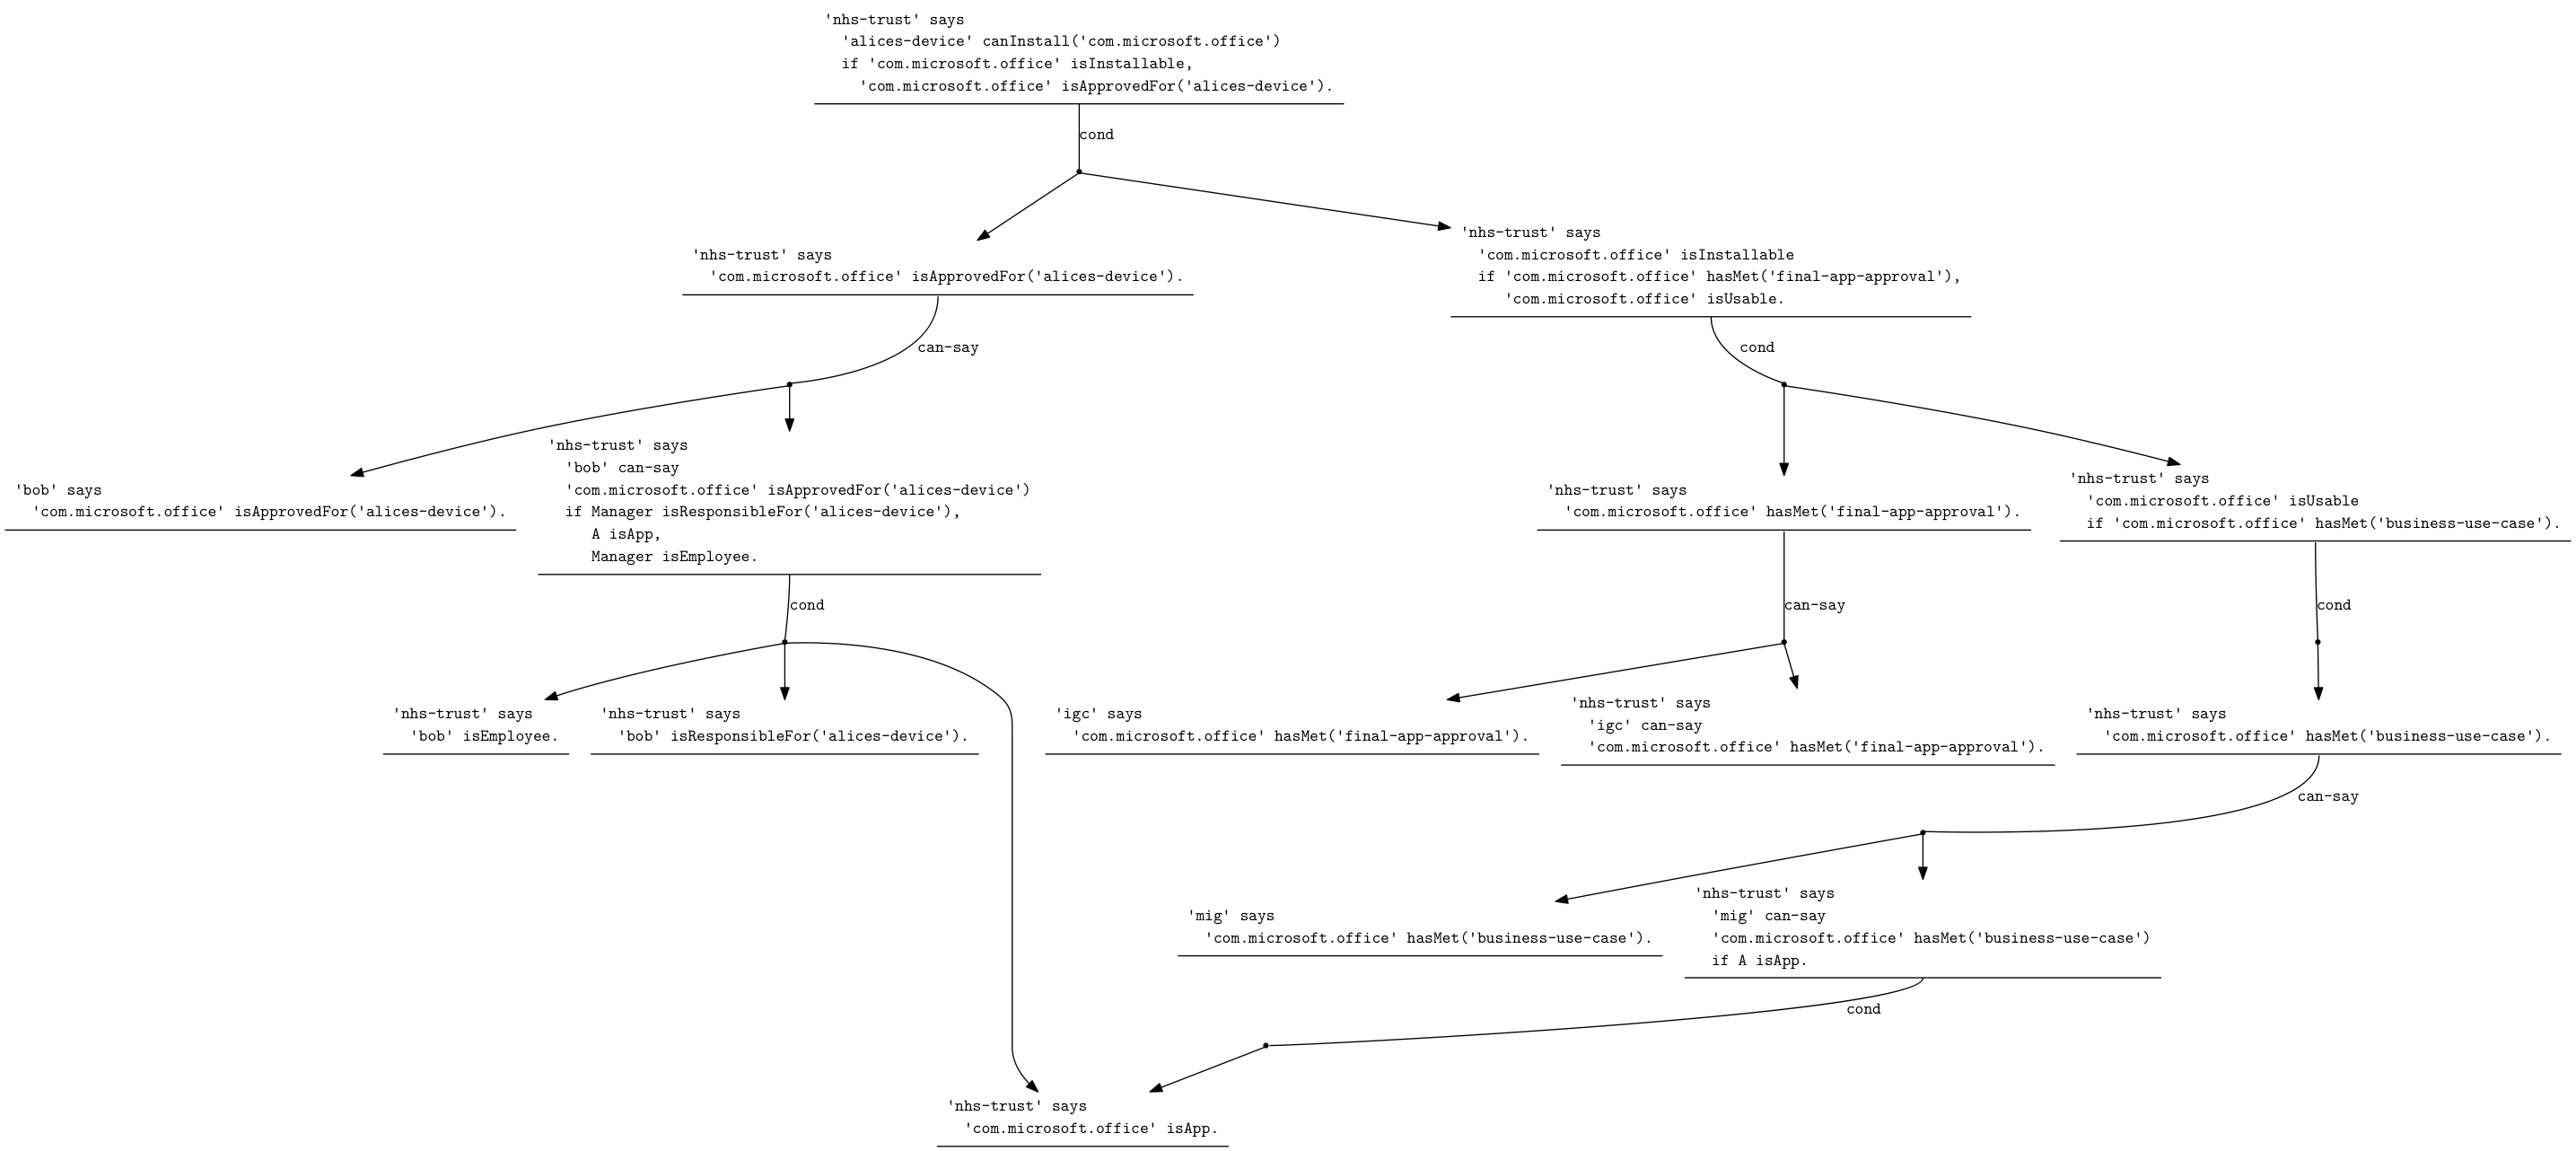
\includegraphics[width=\linewidth]{figures/proof.png}
%  \caption{Proof tree for Alice installing her app.}
%  \label{fig:proof}
%\end{figure}

\section{BYOD Idioms}

When examining the policies, we noticed two particular idioms reappearing: acknowledgements and delegation.
We describe both idioms in greater detail, and show how they can be implemented in \AppPAL{}, below.
MDM tools and research have focussed so far on implementing restrictions on apps and devices~\cite{_ibm_????,armando_formal_2014,martinelli_enhancing_2016}.
Implementing these controls is a vital aspect of BYOD policies and all 5 of the policies we looked at had rules that described restrictions~(\autoref{tab:summary}).
Every policy also contained rules that required employees acknowledgements, however.
Only the SANS policy (which is configuration focussed) contained more rules that required restrictions than acknowledgements. 
All the policies contained more rules featuring delegation relationships than functionality restrictions.
Restricting device functionality is tricky and important, but other aspects of BYOD policies are also worth attention.

\subsubsection{Delegation and Roles within Policies.}

Delegation is an important part of each of the policies.
Each of the policies describes through rules how separate entities may be responsible for making some decisions.
These rules can be a delegation to an employee's manager to authorize a decision (as in the NHS policy). 
It could be to technical staff to decide what apps are part of a standard install (as in the sirens and SANS policies).

\AppPAL~requires an explicit speaker for each assertion.
Speakers can delegate to others by making a statement about what they \emph{can-say}.
When translating the policies, the author of the policy is used as the primary speaker of the policy's rule (\autoref{tab:summary}).
For the \ac{HiMSS} policy, where the user states what they will do rather than the company stating what they must, the user is the primary speaker.
All the policies describe multiple entities that might make assertions and delegate.
With \AppPAL~policies any speaker can delegate a decision to another speaker (with restrictions on re-delegation).
The delegation might be to a user to acknowledge a policy, or it might be to other groups in the company who are responsible for certain decisions.

In all the policies we looked at the majority of the decisions are made by three groups of speakers: 
  the company, the IT-department, and the users or employees.
All the policies also delegate to a user (apart from \ac{HiMSS} where the user is the primary speaker).
The user is typically responsible for providing information, such as agreements to policies, reporting devices missing, and updating passcodes.
In the Sirens, SANS and NHS policy each describe an IT-department who are delegated to make some decisions.
The \ac{HiMSS} policy describes an \emph{xyz-health-system} who act similarly to an IT-department.
These decisions are more varied and can overlap with the responsibilities of the company.
In the NHS and SANS policies, the IT department is responsible for maintaining lists of activated devices.
In the Sirens and SANS policies, the IT department maintains a list of what is installable on a device or not.

%\begin{table}\centering\footnotesize
  %\begin{tabular}{l l}
    %\toprule
    %Policy      & Primary Speaker           \\
    %\midrule
    %{SANS}      & \emph{company}            \\
    %{HiMSS}     & \emph{user}               \\
    %{NHS}       & \emph{nhs-trust}          \\
    %{Edinburgh} & \emph{records-management} \\
    %{Sirens}    & \emph{department}         \\
    %\bottomrule
  %\end{tabular}
  %\label{tab:principals}
  %\caption{Principal Speakers from each of the policies examined.}
%\end{table}

When a policy decision requires input from a third-party delegation is used.
For example, an employee's manager has to authorise an app install.
The SecPAL \emph{can-say} statement is the basis for a delegation. 
We can ask the HR department to state who is someone's manager.
\begin{lstlisting}
'company' says 'hr-department' can-say 
  Employee:E hasManager(Employee:M).
\end{lstlisting}
If we wish to delegate to someone, we can add conditionals to the can-say statement that enforces any relationship between the delegating and delegated parties.
\begin{lstlisting}
'company' says Manager can-say 
  Employee canInstall(App:A)
  if Employee hasManager(Manager).
\end{lstlisting}

\subsubsection{Acknowledgement.}

All the policies looked at require their subjects to be aware and acknowledge certain rules or policies, 
  or that the company may perform certain actions.
For example, the NHS and \ac{HiMSS} policies state that the organisation will wipe devices remotely to protect confidential information a user loses their device.
Both policies also say that employees would lose personal information if they had it on the device and the company needed to erase it.
The employee is required to be aware of this, and in the case of the \ac{HiMSS} policy, agree to hold the company harmless for the loss.

%\begin{center}
%  \noindent
%  %\begin{minipage}{0.49\linewidth}
%    \begin{policyrule}{HiMSS}
%      I agree to hold XYZ Health System harmless for any loss relating to the
%      administration of PDA/Smartphone connectivity to XYZ Health System systems
%      including, but not limited to, loss of personal information stored on a
%      PDA/Smartphone due to data deletion done to protect sensitive information
%      related to XYZ Health System, its patients, members or partners.
%      \normalfont
%      \begin{lstlisting}
%'xyz-health-system' says 'user' mustAcknowledged('data-loss-policy').
%      \end{lstlisting}
%    \end{policyrule}
%  %\end{minipage}
%  %\begin{minipage}{0.49\linewidth}
%    \begin{policyrule}{NHS}
%      Individuals who have personal data of any kind stored on a corporately
%      issued mobile device must be aware that in the event of loss of the device
%      the above data wipe will include removal of all personal data.
%      \normalfont
%      \begin{lstlisting}
%'nhs-trust' says Staff:S can-say
%  S hasAcknowledged('data-loss-policy').
%'nhs-trust' says Staff:S mustAcknowledged('data-loss-policy').
%      \end{lstlisting}
%    \end{policyrule}   
%  %\end{minipage}
%\end{center}

Both the SANS and the siren-company policies use acknowledgements to link to other sets of rules that employees should follow.
These policies are not further specified, and in the case of an acceptable use policy may be hard to enforce automatically.
The SANS policy requires that all employees follow an email security, acceptable use, and an eCommerce-security policy.
The Sirens policy expects an employee to use their devices ethically and abide by an acceptable use policy.
%\begin{policyrule}{SANS}
%  Users MUST agree to the email security/acceptable use policy and eventually to the eCommerce security policy.
%  \begin{lstlisting}
%'company' says Employee:U mustAcknowledged('email-security'). 
%'company' says Employee:U mustAcknowledged('acceptable-use'). 
%'company' says Employee:U mustAcknowledged('ecommerce-security').
%  \end{lstlisting}
%\end{policyrule}
%\begin{policyrule}{Sirens}
%  The employee is expected to use his or her devices in an ethical manner at all times and adhere to the company's acceptable use policy.
%  \begin{lstlisting}
%'department' says Employee:E mustAcknowledged('acceptable-use').
%  \end{lstlisting}
%\end{policyrule}

When there is a (usually separate) set of rules and concerns employees should be aware of acknowledgements are used.
The company may not have wish to enforce these separate rules automatically, however.
For instance, a company may have an ethical policy that says employees should not use devices for criminal purposes.
The company is not interested in, or capable of, defining what is criminal.
They trust their employees to make the right decision and to be aware of the rules.

To implement these in \AppPAL, a policy author creates two rules: 
  the first stating their employees must have acknowledged the policy,
  the second delegating the acceptance of the policy to the employee themselves.
\begin{lstlisting}
'company' says Employee:E mustAcknowledged('policy').
'company' says Employee:E can-say
  E hasAcknowledged('policy').
\end{lstlisting}

\section{Comparison with Existing MDM Software}

It is interesting to compare \AppPAL~to existing MDM~tools such as IBM's MaaS360 and \ac{BES}, both leading MDM packages~\cite{rob_smith_magic_2016}.
Each of these tools supports enforcing and checking compliance policies. 
They do not, however, use policy languages to specify policies; rather they supply canned policies and rules that admins can tweak.

Acknowledgements form a significant portion of the BYOD policies we looked at but are not addressed by the MDM software at all.
MaaS360 can associate users with devices and can assign them into groups.
It can distribute electronic documents, but there are no means to track what policies a user should read and follow.
Administrators could add users who have acknowledged a policy to a group.
One might imagine that users who have acknowledged some additional rules might be added to additional groups with stricter or more relaxed policies, but this is a semi-manual process for an administrator to set up and manage.
One might imagine administrators adding users who have acknowledged some additional rules to new groups
Similarly, with \ac{BES} can create users, groups and groups of devices, but there is no facility for managing what users should agree to automatically.
We can create policies that apply to groups, but not create the groups and policies based on membership of groups.

\AppPAL{} is more flexible than these MDM suites. 
It allows a user to state which policies they have acknowledged and for policies to delegate the acknowledgement of the policy to the user.
We can require that a user must acknowledge certain policies if they meet certain criteria.
Once a statement is made, it can be imported into the \AppPAL~knowledge base and used in making other decisions as part of the policy.

This lack of flexibility extends to trying to compose policies. 
Consider the following rule taken from the SANS policy:
\begin{policyrule}{SANS}
Any non business-owned (that, is private) device must be able to connect to Company network MUST first be approved by technical personnel such as those from the Company IT department or desktop support.
If allowed, privately-owned handheld devices MUST comply with this security policy and MUST be inventoried along with corporate handhelds, but identified as private. This is in order to prevent theft of corporate data with unmanaged handhelds (i.e. owner of device is not identified).
\end{policyrule}
To implement this using an MDM solution such as MaaS360 or \ac{BES} administrators can mark some devices as being privately owned.
A group could be set up for approved privately-owned devices.
MaaS360 allows the creation of groups based on search criteria, though the groups are not dynamic\footnote{The search would need to be re-run when new devices were added or a device's status changed.}.
Technical personnel could be given an administrator login to the MDM software to add devices to this group periodically and could pass them along for inventorying.
Again the management of \emph{who} is \emph{technical personnel} is effectively manual, with optional searches to define groups.
Once we find those devices that can connect we could add an access control rule to a group containing them to enforce the rule.

In \AppPAL~the policy specifies all roles and relationships.
We are free to use conformance to one policy as a conditional for applying a second, allowing dynamic groups.
Roles such as being \emph{technical personnel} can be given to users holding other roles without requiring manual intervention.
Furthermore, the \AppPAL~rule is presented in much the same form as the rule in the policy document: \emph{device} can do \emph{action} if \emph{checks} are satisfied.

\begin{lstlisting}
'company' says Device:D canConnectTo(Network:N)
  if N isCompanyOwned,
     D isPrivatelyOwned,
     D isApproved,
     D hasMet('security-policy').

'company' says 'technical-personnel' can-say
  Device:D isApproved.

'company' says 'it-department' can-act-as 'technical-personnel'.
'company' says 'desktop-support' can-act-as 'technical-personnel'.
\end{lstlisting}

\AppPAL~improves upon existing MDM tools by allowing sophisticated delegation relations and by providing a declarative language for expressing policies.
The language gives greater flexibility to policy authors and allows them to write policies that depend on other policies rather than predefined settings and groups.
It lets us track what users have agreed to, what their policies are, how they are specified, and how they are satisfied.

%\begin{figure}\centering
%  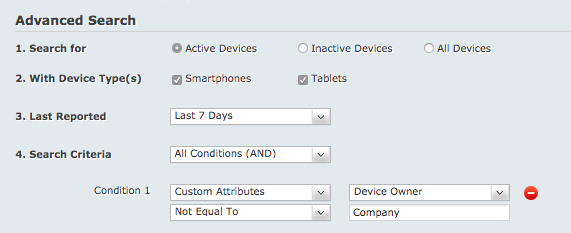
\includegraphics[width=0.5\linewidth]{figures/maas-groupsearch.png}
%  \caption{MaaS360's search interface for devices.}
%  \label{fig:maas360search}
%\end{figure}

\section{Conclusions}
\label{sec:conclusions}
% 1/2 page

We have presented \AppPAL: an instantiation of SecPAL for BYOD policies.
Using an \AppPAL~formalization of 5 BYOD policies we have identified several concerns that existing BYOD tools ignore.
BYOD policies contain delegation and trust relationships that define who is responsible for making different decisions in a company.
Sometimes that is administrators and technical staff deciding what to permit inside the company, and sometimes it is the user's themselves agreeing to follow a policy.
Previous work has focussed on the technical staff's decisions and developing new ways to automate their decisions.
Our work looks at the policies at a higher level tracking, managing and authorizing policies based on what people have said and what tools were run.

Future work will incorporate new BYOD and static analysis tools into \AppPAL. 
This will allow us to use them as part of policy checks.
Whilst earlier work on SecPAL based languages~\cite{becker_secpal:_2010,moritz_y_becker_secpal:_2009} has described how to distribute assertions there has not been a well-defined protocol for doing so.
Future work will also work on tying down the distribution mechanisms and defining the distribution protocol.

%\bibliographystyle{plain}
\printbibliography

\end{document}
